\documentclass[a4paper, 12pt]{article}
\usepackage[utf8]{inputenc}
\usepackage[english]{babel}
\usepackage{graphicx}
\usepackage{hyperref}
\usepackage[a4paper]{geometry}
\usepackage{float}
%\usepackage[left=1cm,right=2cm,vmargin=2.5cm,footnotesep=0.5cm]{geometry}
\usepackage{amssymb,amsmath,amsthm}
\DeclareMathOperator*{\E}{\mathbb{E}}
\DeclareMathOperator*{\Var}{\text{Var}}
\renewcommand*{\P}{\mathbb{P}}
\newtheorem{theorem}{Theorem}
\newtheorem{proposition}{Proposition}
\newtheorem{lemma}{Lemma}

\hypersetup{
    colorlinks=true,
    linkcolor=blue,
    filecolor=magenta,      
    urlcolor=cyan,
    pdftitle={Sharelatex Example},
    bookmarks=true,
    pdfpagemode=FullScreen
}

  
\begin{document} 

\begin{titlepage}
	\centering
	{\scshape\LARGE Ozonmasters \par}
	\vspace{1cm}
	{\scshape\Large Algorithmic Game Theory \par}
	\vspace{1.5cm}
	{\huge\bfseries Home work \par}
	\vspace{2cm}
	{\Large\itshape Kozhemyak Vitaly \par}
	\vfill

% Bottom of the page
	{\large \today\par}
\end{titlepage}
  
\tableofcontents

\newpage
 
\section{Task 1}
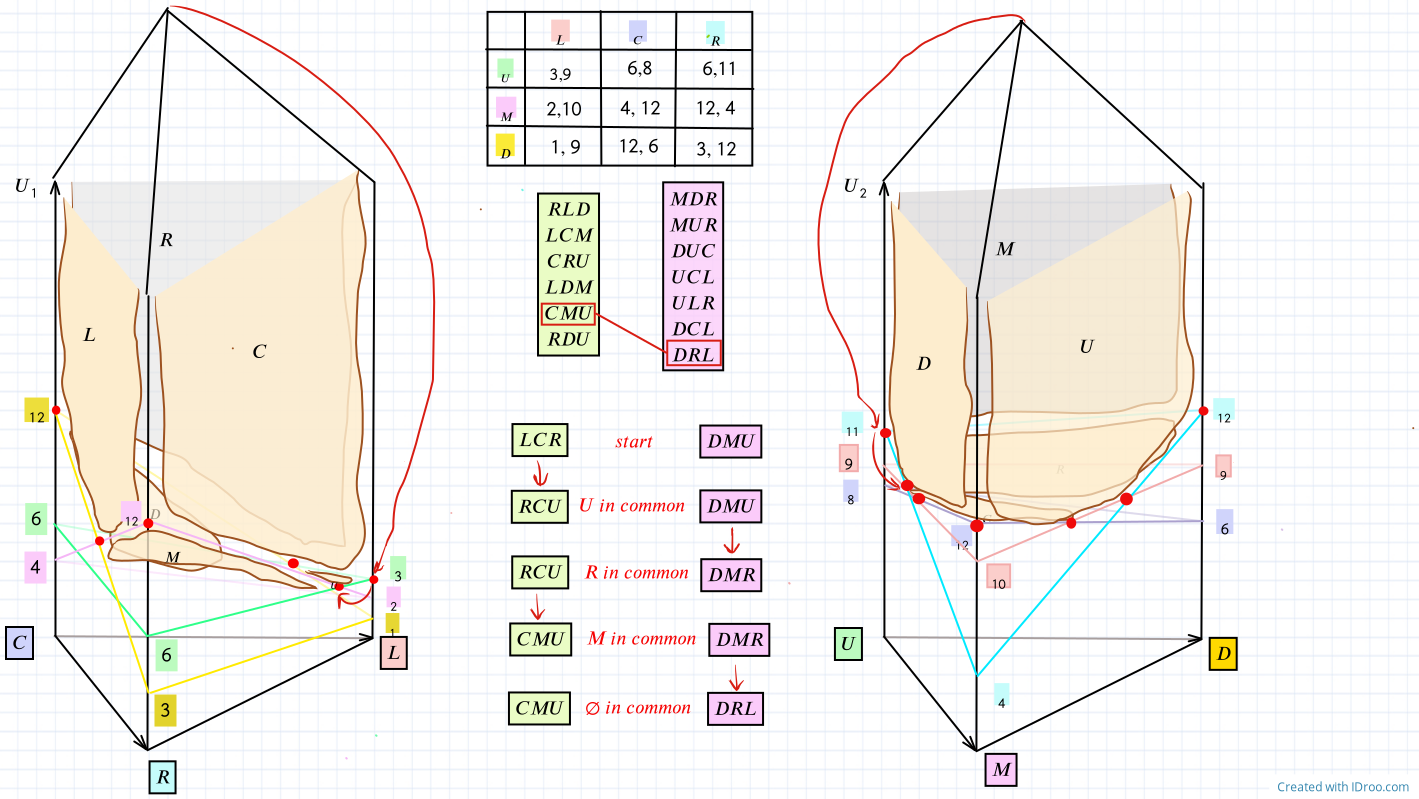
\includegraphics[width=\textwidth]{Images/Task1.png}
\section{Task 3}
Consider two matrix
\begin{center}
\begin{tabular}{|c|c|c|} 
\hline
& L & R\\ [0.5ex] 
\hline
U & (-10, -5) & (6, 0)\\ 
\hline
D & (0, 4) & (0, 0)\\ 
\hline
\end{tabular}
\begin{tabular}{|c|c|c|} 
\hline
& L & R\\[0.5ex]
\hline
U & $\P (U, L) = \alpha$ & $\P (U, R) = \beta$\\ 
\hline
D & $\P (D, L) = \gamma$ & $\P (D, R) = \delta$\\ 
\hline
\end{tabular}
\end{center}
It's easy to see that there are two pure strategies: $E(U, R) = (6, 0), E(D, L) = (0, 4).$\\
\noindent Also there is one mixed strategy $E \left( \dfrac{4}{9} U + \dfrac{5}{9} D, \dfrac{3}{8} L + \dfrac{5}{8} R \right) = (0, 0).$\\
\noindent Suppose the first player obeys the rules. It could happen when
$$
\begin{cases}
-10 \dfrac{\alpha}{\alpha + \beta} + 6 \dfrac{\beta}{\alpha + \beta} \geqslant 0 \\
0 \geqslant -10 \dfrac{\gamma}{\gamma + \delta} + 6 \dfrac{\delta}{\gamma + \delta}
\end{cases}
\Leftrightarrow
\begin{cases}
3 \beta \geqslant 5 \alpha, \\
5 \gamma \geqslant 3 \delta.
\end{cases}
$$
Suppose the second player obeys the rules. It could happen when
$$
\begin{cases}
-5 \dfrac{\alpha}{\alpha + \gamma} + 4 \dfrac{\gamma}{\alpha + \gamma} \geqslant 0 \\
0 \geqslant -5 \dfrac{\beta}{\beta + \delta} + 4 \dfrac{\delta}{\beta + \delta}
\end{cases}
\Leftrightarrow
\begin{cases}
4 \gamma \geqslant 5 \alpha, \\
5 \beta \geqslant 4 \delta.
\end{cases}
$$
Now consider the worst and better cases.
\begin{itemize}
	\item The worst case of correlated strategy is attained on the solution of the next system of equations
$$
\begin{cases}
4 \gamma = 5 \alpha, \\
5 \beta = 4 \delta, \\
3 \beta = 5 \alpha, \\
5 \gamma = 3 \delta, \\
\alpha + \beta + \gamma + \delta = 1,
\end{cases}
\Rightarrow
\alpha = \dfrac{1}{6}, \beta = \dfrac{5}{18}, \gamma = \dfrac{5}{24}, \delta = \dfrac{25}{72}.
$$
The expected payoff of the first player $E_1 = -10 \alpha + 6 \beta = 0.$\\
The expected payoff of the second player $E_2 = -5 \alpha + 4 \gamma = 0.$
	\item But we can get better if we put $\alpha = 0$ and solve the next system of equation
$$
\begin{cases}
5 \beta = 4 \delta, \\
5 \gamma = 3 \delta, \\
\beta + \gamma + \delta = 1,
\end{cases}
\Rightarrow
\beta = \dfrac{1}{3}, \gamma = \dfrac{1}{4}, \delta = \dfrac{5}{12}.
$$
The expected payoff of the first player $E_1 = -10 \alpha + 6 \beta = 2.$\\
The expected payoff of the second player $E_2 = -5 \alpha + 4 \gamma = 1.$\\
We can see the expected payoff of this correlated strategy is grater than the expected payoff of the mixed strategy.
	\item But we go further and put $\alpha = \delta = 0.$ Solve the next equation
$$
\beta + \gamma = 1
\Rightarrow
\beta = 1 - \gamma, 0 \leqslant \gamma \leqslant 1.
$$
Thus, the solution is the whole segment connecting two pure strategies in the coordinate plane $(E_1, E_2).$\\
The expected payoff of the first player $E_1 = -10 \alpha + 6 \beta = 6 - 6 \gamma, 0 \leqslant \gamma \leqslant 1.$\\
The expected payoff of the second player $E_2 = -5 \alpha + 4 \gamma = 4 \gamma, 0 \leqslant \gamma \leqslant 1.$\\
If we put $\gamma = \dfrac{1}{2}$ then $E_1 = 3, E_2 = 2.$ We can see the expected payoff of this correlated strategy is grater than the expected payoff of the previous one.
\end{itemize}
\begin{figure}[H]
\centering
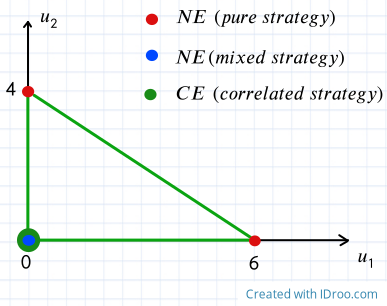
\includegraphics[width=\textwidth]{Images/Task3.png}
\caption{A coordinate plane of expected payoff. Set of correlated strategies is the whole green triangle including interior and boundaries.}
\end{figure}
\section{Task 4}
Consider an atomic (i.e. there
are finitely many players controlling a non-negligible amount of traffic) instance which is defined by a triple of the form $(G, r, c),$ with $G$ the directed graph, $r$ the amount of traffic of each
commodity (i.e. pair $(s, t)$ where $s$ --- start of the path, $t$ --- end of the path) and $c$ the cost functions of all edges. 

Player $i$’s cost function, given a strategy $s$ with corresponding flow $f,$ is
$$
	Cost_i(f) = r_i \cdot c_{s_i}(f) = r_i \cdot \sum \limits_{e \in s_i} c_e(f_e).
$$
The cost of a flow $f$ is given by
$$
C(f) = \sum \limits_{i=1}^N Cost_i(f)
$$
where $N$ --- number of players.
\begin{enumerate}
	\item AAE example. Consider an unweighted (all $r_i$ are equal) atomic instance with two Nash flows that have different costs. Each player
has the same traffic rate, $r = 1,$ and the Price of Anarchy is 
$$
\dfrac{C(f_{Nash})}{C(f_{opt})} = \dfrac{3 + 3 + 2 + 2}{1 + 1 + 1 + 1} = \dfrac{5}{2},
$$
 If we set the
traffic rate for players 1 and 2 to $\dfrac{1 + \sqrt{5}}{2}$ (the golden ratio) and the traffic
rate for the other players to 1, then the Price of Anarchy is 
$$
\dfrac{C(f_{Nash})}{C(f_{opt})} = \dfrac{3 \cdot \dfrac{1 + \sqrt{5}}{2} + 3 \cdot \dfrac{1 + \sqrt{5}}{2} + 2 + 2}{2 \cdot \dfrac{1 + \sqrt{5}}{2} + 2 \cdot \dfrac{1 + \sqrt{5}}{2} + 1 + 1} = \dfrac{3 + \sqrt{5}}{2},
$$ which
is the highest possible Price of Anarchy for atomic instances with affine cost functions. 
	\item Consider the next atomic instance $(G, r, c)$ with three players. Set $r_i = 1, \forall i \in \{1, 2, 3\}.$ 
	
The optimal strategies are for each player to move in a straight line. 
\begin{figure}[H]
\centering
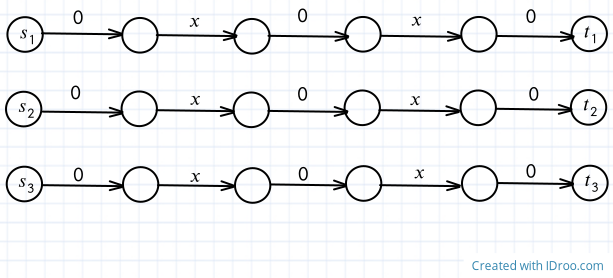
\includegraphics[width=\textwidth]{Images/Task4_2.png}
\caption{The optimal player's strategies.}
\end{figure}
At the Nash equilibrium each player moves according to his own color. The bold (non-dashed) means the path cost is $c(x) = x,$ the dashed line means the path cost is $c(x) = 0.$
\begin{figure}[H]
\centering
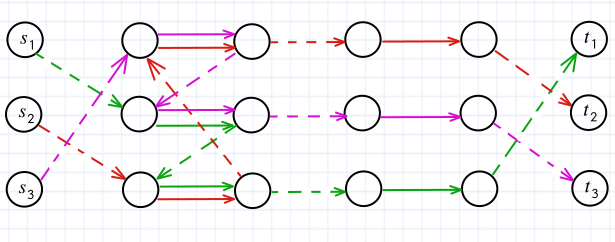
\includegraphics[width=\textwidth]{Images/Task4_2_1.png}
\caption{Nash equilibrium. The bold (non-dashed) means the path cost is $c(x) = x,$ the dashed lines means the path cost is $c(x) = 0.$}
\end{figure}
We can calculate the Price of Anarchy as follows
$$
\dfrac{C(f_{Nash})}{C(f_{opt})} = \dfrac{5 + 5 + 5}{2 + 2 + 2} = \dfrac{5}{2}.
$$
\item There are no any ideas.
\item At the lecture one theorem about the price of anarchy in affine weighted atomic instances was mentioned. 
\begin{theorem}
If $(G, r, c)$ is an atomic instance with affine cost functions, then the price of anarchy of $(G, r, c)$ is at most $\dfrac{3 + \sqrt{5}}{2} \approx 2.618.$
\end{theorem}
\end{enumerate}

\section{Task 5}
Below we describe the \textbf{Cut Your Own Piece (CYOP) protocol} for $n$ players.\\
\fbox{
\begin{minipage}{35em}
\textbf{Given:}
\parbox[t]{30em}{
Cake $X = [0, 1]$ and players $p_1, \ldots, p_n.$
}\\
\textbf{Step 1:}
\parbox[t]{30em}{
Every player makes $n-1$ markings to divide the cake into $n$ pieces of a value $\dfrac{1}{n}$ (according to their valuation function). All $n(n-1)$ markings are required to be in parallel to the left and right edge of the cake, and no player knows the markings of the other player.
}\\\\
\textbf{Step 2:}
\parbox[t]{30em}{
Identify the leftmost marking.
\begin{itemize}
	\item The piece of cake between the left edge of the cake and the leftmost marking is assigned to any of the players that placed a marking at this position and this player drops out.
	\item Remove all markings of the player just dropped out as well as the leftmost markings of all remaining players.
\end{itemize}
}\\\\
\textbf{Step 3:}
\parbox[t]{30em}{
Repeat Step 2 for all remaining players and the remaining cake until all markings have been removed.
}\\\\
\textbf{Step 4:}
\parbox[t]{30em}{
The last remaining player receives the remaining cake. 
}
\end{minipage}
}\\\\
\noindent Now we are going to proof some properties of the algorithm.
\begin{proposition}
Suppose that at least two of the $n$ players in the CYOP protocol have made distinct markings. Then the cake can be divided such that
\begin{enumerate}
	\item all players received a piece that they themselves have marked,
	\item no two of these pieces overlap, 
	\item a nonempty piece remains.
\end{enumerate} 
\end{proposition}
\begin{proof}
We prove this think by induction on $n.$ The induction base, $n= 2,$ is easy to see: if two players disagree by making distinct markings, we can assign them disjoint pieces of the cake that they have marked themselves, and a nonempty piece remains between the two markings. 

For the induction step assume the claim to be true for $n$ players. To show it for $n + 1$ players, suppose that $p_1, \ldots, p_{n+1}$ have made their markings according to the CYOP protocol. Cut at the leftmost marking and assign the piece left of the cut to the player who made this marking, where ties can be broken arbitrarily. Without loss of generality, assume that $p_1,$ gets this piece and drops out. Now, remove all markings of $p_1,$ and also the leftmost markings of all other players $p_i, i \neq 1.$ By induction hypothesis, all the players $p_2, \ldots p_{n+1}$  receive piece that they themselves have marked, and no two of these pieces overlap. 

To prove that a nonempty piece of the cake remains, consider the following two cases.
\begin{enumerate}
	\item There are players $p_i$ and $p_j, 2 \leqslant i, j \leqslant n + 1$ and $i \neq j,$ whose remaining markings do not coincide. By induction hypothesis, a nonempty piece of cake remains. 
	\item For all players $p_i$ and $p_j, 2 \leqslant i, j \leqslant n + 1$ and $i \neq j,$ all remaining markings coincide. Consider the following two subcases.
\begin{enumerate}
	\item The disagreement of our original assumption for $n+1$ players concerned the leftmost markings only. Thus, there exists some $i, 2 \leqslant i \leqslant n + 1,$ such that $p_i$ would get more than he originally has marked. Assign to $p_i$  his originally marked piece instead. A nonempty piece of the cake remains. (All other pieces can be arbitrarily assigned to the other players, due to their markings being identical).
	\item The leftmost markings of the players coincided. That is the disagreement of our original assumption for $n+1$ players concerned their other (not their leftmost) piece markings only. In that case, assign the first (the leftmost) piece not to $p_1,$  but, for instance,  to $p_2.$ We then are again in case (a).
\end{enumerate}
\end{enumerate}
It is fairly may to see that the CYOP protocol is proportional and immune to manipulation for risk-averse players, i.e. envy-free protocol. All players are guaranteed to receive a proportional share. However, if a player try to cheat he is jeopardizing to receive a proportional share himself (but this does not have any impact on any other player's guaranteed proportional share). For example, a cheating player might place his marks such that some of his marked pieces is worth more than $\dfrac{1}{n},$ hoping to receive this particular piece. However, this also means, that at least one of his marked pieces is worth less than $\dfrac{1}{n}.$ Because the players cannot directly influence which piece they are going to get assigned (as this always also depends on he other player's markings which are unknown), the cheating player may end up with even less than a proportional share.    
 
\end{proof}
\end{document} 